\documentclass[conference]{IEEEtran}
\IEEEoverridecommandlockouts
\usepackage[T1]{fontenc}
\usepackage{mathptmx}
\usepackage{amsmath,amssymb}
\usepackage{graphicx}
\usepackage{booktabs}
\usepackage{multirow}
\usepackage{array}
\usepackage{xcolor}
\usepackage{url}
\usepackage[hidelinks]{hyperref}
\usepackage{cite}
\graphicspath{{figures/}}
\newcommand{\sig}[1]{\texttt{\small #1}}
\renewcommand{\arraystretch}{1.12}
\renewcommand{\topfraction}{0.92}\renewcommand{\bottomfraction}{0.8}\renewcommand{\textfraction}{0.06}
\renewcommand{\floatpagefraction}{0.75}\renewcommand{\dbltopfraction}{0.92}\renewcommand{\dblfloatpagefraction}{0.75}
\setcounter{topnumber}{3}\setcounter{dbltopnumber}{2}\setcounter{totalnumber}{5}

\begin{document}

\title{Instruction and Data Memory Hierarchy: A Harvard-Style Memory Organization in Verilog and a Fair Comparison with a Shared-Memory Baseline}

\author{
\IEEEauthorblockN{Aadit Vachher, Kush Puri, Aabir Sarkar, Kushagra Maheshwari, Kavya Katal}
\IEEEauthorblockA{\textit{Team Lethals --- Modern Computer Architecture, Project 9}\\
\textit{Newton School of Technology, Rishihood University}, Sonipat, India\\
Repository: \url{https://github.com/KatalKavya96/Lethals_MCA_Project}}
}

\maketitle

% ------------------------------------------------------------------
\begin{abstract}
A processor that keeps instructions and data in one memory behind one port can either fetch an instruction or access data in a given cycle, never both. This is the von Neumann bottleneck. A Harvard organization removes the conflict by giving instructions and data separate memories and buses. We implement a simplified Harvard memory organization in synthesizable Verilog: a program counter, an instruction ROM, a data RAM, an address decoder, read/write control, a memory-mapped output register, and a single-cycle accumulator controller. We compare it against a shared-memory baseline that runs the same six-instruction ISA, the same programs and the same data address map. The baseline is built to be fair: it spends a second cycle only on instructions that actually need the port for data. Directed testbenches check 71 conditions across unit and system level, and both designs produce identical final memory, accumulator and output values. Measured cycle counts follow the analytical model exactly: $N$ cycles for Harvard and $N+M$ for the shared design, where $M$ of the $N$ executed instructions access data memory. The resulting speed-ups are $1.72\times$, $1.69\times$ and $1.25\times$ on three programs, so the gain is $1+M/N$ and not a fixed $2\times$. Generic Yosys synthesis gives nearly equal cell counts (17\,481 vs.\ 17\,471), which we show is a consequence of the chosen memory sizes. The Harvard critical path is slightly deeper (33 vs.\ 31 gate levels) because it chains an instruction read into a data read within one cycle. We state clearly that the speed-up is a cycle-count result: maximum frequency has not yet been measured on an FPGA, and that is the main goal of Phase II.
\end{abstract}

\begin{IEEEkeywords}
Harvard architecture, von Neumann bottleneck, memory organization, address decoding, Verilog RTL, finite-state machine, cycle-accurate simulation, logic synthesis.
\end{IEEEkeywords}

% ------------------------------------------------------------------
\section{Introduction}
Every instruction a processor executes must first be fetched from memory, and many instructions then read or write data in memory as well. Where those two kinds of access go, and whether they can happen at the same time, is one of the oldest decisions in computer organization. The stored-program design described by von Neumann~\cite{vonneumann} keeps instructions and data in the same memory. This is flexible and economical, but it forces fetches and data accesses to take turns on one path. Backus later called that path ``the von Neumann bottleneck''~\cite{backus}. The Harvard Mark~I~\cite{aiken} took the opposite approach, with physically separate stores for instructions and data.

Project~9 of our Modern Computer Architecture course asks us to ``implement a simplified Harvard-style memory organization with separate instruction and data paths and analyze its behavior,'' and to compare it with a shared-memory organization. The evaluation focuses on correct instruction/data separation, memory control, timing behaviour and the architecture comparison. This report makes the following contributions:
\begin{enumerate}
\item A modular, synthesizable Verilog implementation of both organizations. They share the same program counter, read/write control, output register and ISA, so the memory organization is the only thing that differs (Section~\ref{sec:proposed}).
\item A \emph{fair} shared-memory baseline. It is charged an extra cycle only for instructions that need the port for data, and it turns ``analyze simultaneous access opportunities'' into a measurable quantity, $f=M/N$.
\item Directed verification at unit and system level, with waveform evidence taken from the simulation itself (Section~\ref{sec:verif}).
\item Measured cycle counts, an analytical model that predicts them exactly, generic synthesis results, and an honest account of what these numbers do and do not show (Sections~\ref{sec:results}--\ref{sec:discussion}).
\end{enumerate}

% ------------------------------------------------------------------
\section{Literature Review}\label{sec:lit}

\subsection{The stored-program machine and its bottleneck}
Von Neumann's EDVAC report~\cite{vonneumann} placed the program in the same memory as the data it operates on. This made programs modifiable data and greatly simplified the hardware. The cost appears whenever the processor needs both an instruction and an operand: a single memory port can deliver only one word per access. Backus~\cite{backus} named this the von Neumann bottleneck and argued that it limits both hardware throughput and programming style. Fig.~\ref{fig:concept}(a) shows the organization.

\begin{figure}[!t]
\centering
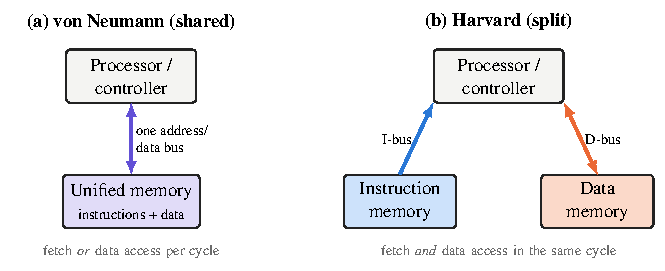
\includegraphics[width=\columnwidth]{concept.pdf}
\caption{The two organizations compared in this project. (a)~One memory and one bus: each cycle carries either a fetch or a data access. (b)~Separate instruction and data memories and buses: both can be used in the same cycle.}
\label{fig:concept}
\end{figure}

\subsection{Harvard and modified-Harvard organizations}
The Harvard Mark~I read instructions from punched tape and kept data in separate electromechanical counters~\cite{aiken}. In modern designs the idea survives in two main forms. Digital signal processors adopted strict or modified Harvard buses so that an instruction and one or more operands can be read every cycle, which is essential for sustained multiply--accumulate throughput~\cite{eyre}. Most general-purpose processors are \emph{modified} Harvard machines. Main memory is unified, as in the von Neumann model, but the first cache level is split into an instruction cache and a data cache, so the pipeline can fetch and access data in the same cycle~\cite{hennessy,smith}. Smith's survey of cache memories discusses this split and its trade-offs against a unified cache: a split cache doubles the bandwidth and avoids conflicts between the two streams, while a unified cache uses its capacity more flexibly~\cite{smith}. The ``optional shared lower-level memory'' in our project brief corresponds to this modified-Harvard arrangement.

\subsection{Textbook single-cycle datapaths}
Standard teaching datapaths, including the single-cycle MIPS processor covered in our course, draw separate instruction and data memories precisely so that every instruction can finish in one clock cycle~\cite{patterson,harris}. The textbooks note the cost: the clock period must cover the slowest instruction, which includes an instruction-memory read followed by a data-memory read. When the same textbooks move to a multi-cycle design with one memory, the instruction and data accesses are spread over separate cycles. Our two designs are a minimal version of this pair, with the datapath reduced to an accumulator so that the memory organization stays the focus.

\subsection{The memory wall and Amdahl's Law}
Wulf and McKee observed that processor speed was growing much faster than memory speed, so memory access would come to dominate execution time, a problem they called the ``memory wall''~\cite{wulf}. Separating instruction and data paths is one of the oldest ways of adding memory bandwidth. Amdahl's Law~\cite{amdahl} reminds us that any speed-up applies only to the part of the work it affects. In our setting, only instructions that touch data memory can benefit from a separate data path. Section~\ref{sec:model} makes this exact.

\subsection{RTL design and verification practice}
We follow IEEE~1364 Verilog~\cite{ieee1364} with synthesizable coding conventions~\cite{palnitkar}. Simulation and synthesis tools may interpret the same source differently. Mills and Cummings catalogue coding styles that cause such simulation/synthesis mismatches~\cite{mills}, and we met one in practice (Section~\ref{sec:mismatch}). FPGA block RAMs register their read address and return data one clock edge later~\cite{ug473}. A memory written with a purely combinational read therefore cannot be mapped onto them, and this affects how our synthesis numbers should be read. We use Icarus Verilog~\cite{icarus}, GTKWave~\cite{gtkwave} and Yosys~\cite{yosys}.

\subsection{Gap addressed}
Textbooks usually present Harvard and von Neumann organizations qualitatively, or compare a single-cycle machine against a multi-cycle machine that differs in many other ways. Course-level ``Harvard vs.\ von Neumann'' demonstrations often charge the shared design two cycles for \emph{every} instruction, which produces a $2\times$ speed-up by construction. We instead keep everything except the memory organization identical. This lets the speed-up be predicted from the instruction mix, and then measured.

% ------------------------------------------------------------------
\section{Proposed Solution}\label{sec:proposed}

\subsection{Design rules for a fair comparison}\label{sec:rules}
We fixed the following rules before writing any RTL. Both designs:
\begin{enumerate}
\item execute the \emph{same} ISA and the \emph{same} program files;
\item present the \emph{same} logical data address map to the program;
\item use memories with the \emph{same} timing (synchronous write, combinational read);
\item reuse the \emph{same} \sig{pc}, \sig{rw\_control} and \sig{out\_reg} modules;
\item count cycles with the \emph{same} rule: every rising edge while out of reset and not yet done, with HALT counted.
\end{enumerate}
The shared baseline takes a second cycle \emph{only} for instructions that use the port for data. Charging it for unneeded EXEC cycles would inflate the Harvard advantage.

\subsection{Instruction set and format}
A pure load/store ISA would make every non-HALT instruction a memory access, and then the speed-up would be the same for every program. We therefore added an accumulator and two instructions that do not access data memory (LDI and NOP), so programs can mix memory and non-memory work. Table~\ref{tab:isa} lists the six instructions and Fig.~\ref{fig:format} the 32-bit word format.

\begin{table}[!t]
\caption{Instruction set (accumulator machine)}
\label{tab:isa}
\centering
\begin{tabular}{@{}clll@{}}
\toprule
Op & Name & Action & Data memory \\
\midrule
0 & NOP   & none                            & --- \\
1 & LOAD  & ACC $\leftarrow$ M[addr]        & read \\
2 & STORE & M[addr] $\leftarrow$ ACC        & write \\
3 & LDI   & ACC $\leftarrow$ imm (zero-ext.) & --- \\
4 & ADD   & ACC $\leftarrow$ ACC + M[addr]  & read \\
F & HALT  & done $\leftarrow$ 1, PC holds   & --- \\
\bottomrule
\end{tabular}
\end{table}

\begin{figure}[!t]
\centering
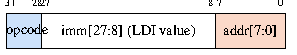
\includegraphics[width=0.95\columnwidth]{instr_format.pdf}
\caption{Instruction word. \sig{addr} is a data-space \emph{offset}, so the same program runs unchanged on both designs.}
\label{fig:format}
\end{figure}

\subsection{Address map and decoding}
Fig.~\ref{fig:memmap} shows both address maps. In the Harvard design the instruction ROM has its own address space, and the data-side decoder selects data RAM for offsets \texttt{0x00}--\texttt{0x6F} and a memory-mapped OUT register at \texttt{0x70}. Writes elsewhere are ignored and reads return zero. In the shared design the program occupies \texttt{0x00}--\texttt{0x7F} of the single memory. The controller adds a base of \texttt{0x80} to every data offset, so the program sees exactly the same data map. The shared decoder also \emph{blocks data writes into the program region}. Without this, offset \texttt{0x90} would wrap to absolute \texttt{0x10} and overwrite an instruction. Program P3 tests this case deliberately.

\begin{figure}[!t]
\centering
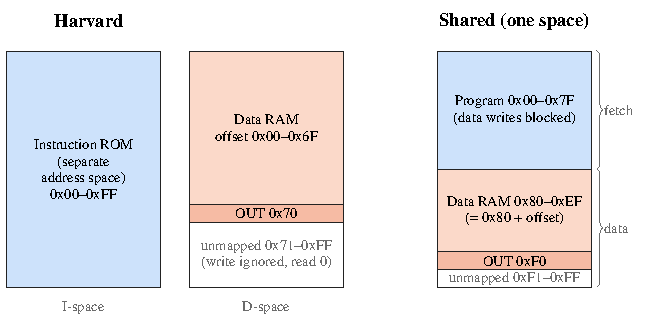
\includegraphics[width=\columnwidth]{memmap.pdf}
\caption{Address maps. Harvard has two independent spaces. The shared design has one space, and the decoder separates program and data regions.}
\label{fig:memmap}
\end{figure}

\subsection{Harvard organization}
Fig.~\ref{fig:blockh}(a) shows the Harvard design. The instruction bus (PC $\rightarrow$ ROM $\rightarrow$ controller) and the data bus (controller $\leftrightarrow$ decoder $\leftrightarrow$ RAM/OUT) share no wire. Every instruction completes in one cycle. Within one clock period the PC addresses the ROM, the opcode is decoded combinationally, the \sig{addr} field addresses the data RAM, and the accumulator and RAM are updated on the closing edge (Fig.~\ref{fig:datapath}). The only clocked state is PC, ACC, \sig{done}, the OUT register and the RAM array. The address decoder sits only on the data side, because anything placed on both paths would reintroduce the conflict the design is meant to remove.

\begin{figure*}[!t]
\centering
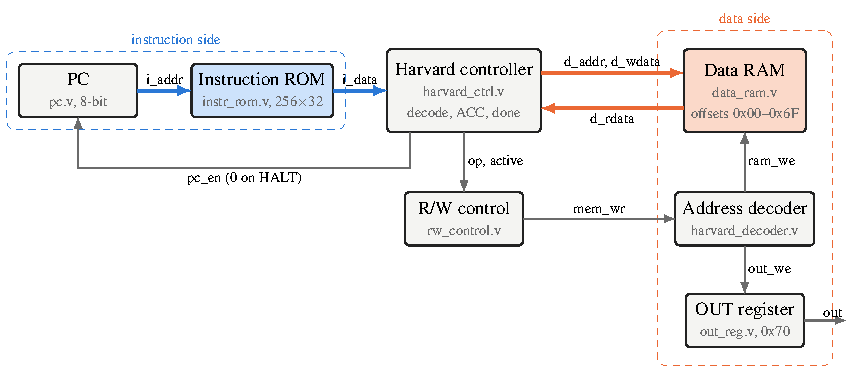
\includegraphics[width=0.8\textwidth]{block_harvard.pdf}\\[1mm]
{\footnotesize (a) Harvard design (\sig{harvard\_top.v}): instruction side (blue) and data side (orange) never share a wire; the decoder serves only the data side.}\\[3mm]
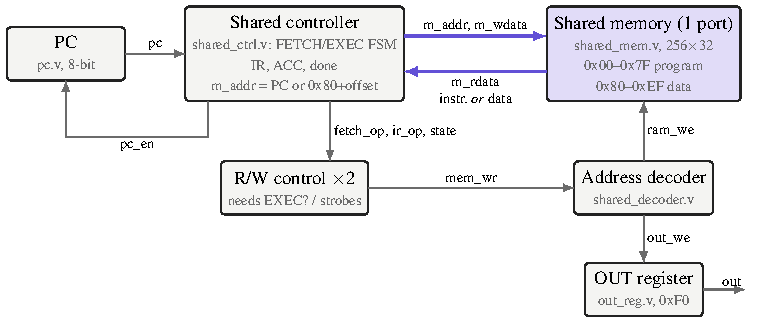
\includegraphics[width=0.8\textwidth]{block_shared.pdf}\\[1mm]
{\footnotesize (b) Shared-memory baseline (\sig{shared\_top.v}): one bus (purple) carries fetches and data accesses in turn.}
\caption{Block diagrams of the two designs. Both reuse the same \sig{pc}, \sig{rw\_control} and \sig{out\_reg} modules.}
\label{fig:blockh}
\end{figure*}

\begin{figure}[!t]
\centering
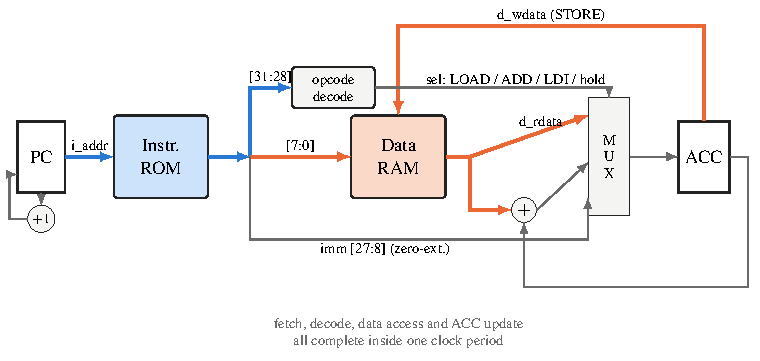
\includegraphics[width=\columnwidth]{datapath_harvard.pdf}
\caption{Harvard single-cycle datapath. The ACC multiplexer selects \sig{d\_rdata} (LOAD), ACC+\sig{d\_rdata} (ADD), the immediate (LDI) or holds. STORE drives ACC onto \sig{d\_wdata}.}
\label{fig:datapath}
\end{figure}

\subsection{Shared-memory baseline}
Fig.~\ref{fig:blockh}(b) shows the baseline: one $256\times32$ memory with one address port. The controller is a two-state Moore FSM (Fig.~\ref{fig:fsm}). In FETCH the port carries the PC and the returned word is the instruction. NOP, LDI and HALT finish in FETCH. LOAD, STORE and ADD latch the word into the instruction register (IR) and move to EXEC, where the port carries \texttt{0x80}+IR[7:0] and the data access happens. The same \sig{rw\_control} module is instantiated twice. The first copy asks whether the fetched instruction needs a second cycle, and the second drives the real strobes in EXEC.



\begin{figure}[!t]
\centering
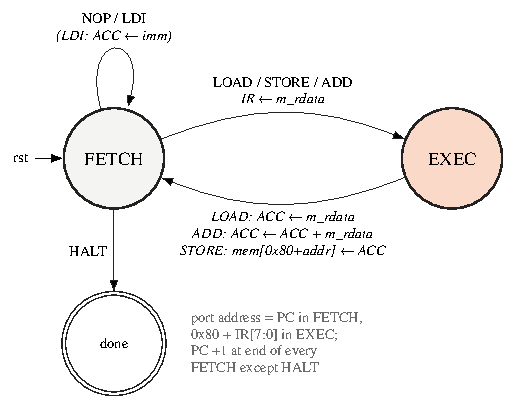
\includegraphics[width=0.92\columnwidth]{fsm_shared.pdf}
\caption{State diagram of the shared controller (\sig{shared\_ctrl.v}). EXEC is entered only for instructions that need the port for data.}
\label{fig:fsm}
\end{figure}

\subsection{Analytical cycle model}\label{sec:model}
Let a program execute $N$ instructions (HALT included), of which $M$ are LOAD, STORE or ADD. With the counting rule of Section~\ref{sec:rules},
\begin{equation}
T_H = N,\qquad T_S = N + M,\qquad S = \frac{T_S}{T_H} = 1 + f,\quad f=\frac{M}{N}.
\label{eq:model}
\end{equation}
The speed-up is bounded by $1 \le S \le 2$. It reaches $2$ only if every instruction accesses data memory, and it falls to $1$ for a program with no data accesses. This is Amdahl's Law~\cite{amdahl} applied to memory-port occupancy: the separate data path helps only the fraction $f$ of instructions that would otherwise compete for the port. The model predicts cycles, not time. Execution time is $T\cdot t_\text{clk}$, and Section~\ref{sec:cp} discusses $t_\text{clk}$.

\subsection{Implementation}
Table~\ref{tab:modules} lists the modules required by the brief and where each is implemented, and Fig.~\ref{fig:hier} shows the instance hierarchy. All modules use one global clock, synchronous active-high reset, and nonblocking assignments in clocked blocks. Programs are hex files loaded with \sig{\$readmemh}. The three test programs are P1, a block copy that writes four values and copies them (memory-heavy, $N{=}18$, $M{=}13$); P2, an array sum with back-to-back reads and a read-after-write ($N{=}16$, $M{=}11$); and P3, mostly non-memory instructions plus a deliberately blocked write ($N{=}16$, $M{=}4$).

\begin{table}[!t]
\caption{Brief's suggested modules and their implementation}
\label{tab:modules}
\centering
\small
\begin{tabular}{@{}p{2.3cm}p{5.4cm}@{}}
\toprule
Module (brief) & File(s) and role \\
\midrule
Program Counter & \sig{pc.v}: 8-bit counter with enable, holds on HALT \\
Instruction Memory & \sig{instr\_rom.v} (Harvard), lower half of \sig{shared\_mem.v} \\
Data Memory & \sig{data\_ram.v} (Harvard), upper half of \sig{shared\_mem.v} \\
Address Decoder & \sig{harvard\_decoder.v}, \sig{shared\_decoder.v} \\
Read/Write Control & \sig{rw\_control.v}: opcode $\rightarrow$ \sig{mem\_rd}/\sig{mem\_wr}, gated by \sig{active} \\
Controller & \sig{harvard\_ctrl.v} (1 cycle), \sig{shared\_ctrl.v} (FSM) \\
Output & \sig{out\_reg.v}: memory-mapped result register \\
\bottomrule
\end{tabular}
\end{table}

\begin{figure}[!t]
\centering
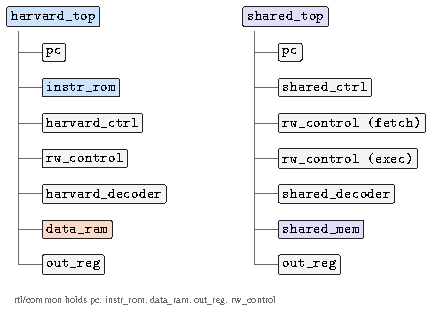
\includegraphics[width=0.85\columnwidth]{hierarchy.pdf}
\caption{Module instance hierarchy of the two top levels.}
\label{fig:hier}
\end{figure}

% ------------------------------------------------------------------
\section{Verification Methodology}\label{sec:verif}
Fig.~\ref{fig:toolchain} shows the toolchain and Fig.~\ref{fig:verif} the verification flow. Verification is directed and self-checking at two levels.

\emph{Unit level} (\sig{tb\_units.v}, 37 checks): \sig{rw\_control} for all six opcodes and with \sig{active} low; both decoders at every boundary address (\texttt{0x6F}/\texttt{0x70}/\texttt{0x71} and \texttt{0x7F}/\texttt{0x80}/\texttt{0xEF}/\texttt{0xF0}/\texttt{0xF1}); PC reset, count and hold.

\emph{System level} (\sig{tb\_harvard.v}, \sig{tb\_shared.v}, 17 checks each): every testbench instantiates the design three times, once per program, and compares final RAM contents, the OUT register, the accumulator, the blocked write and the cycle count against hand-computed values. The shared checks use absolute addresses (\texttt{0x80}+offset) and are otherwise identical.

All 71 checks pass on Icarus Verilog 12 in our environment and on a team member's macOS installation. Waveforms (VCD) are dumped for every run. Fig.~\ref{fig:waveh} is plotted directly from those VCD files, sampled just before each rising edge.

\begin{figure}[!t]
\centering
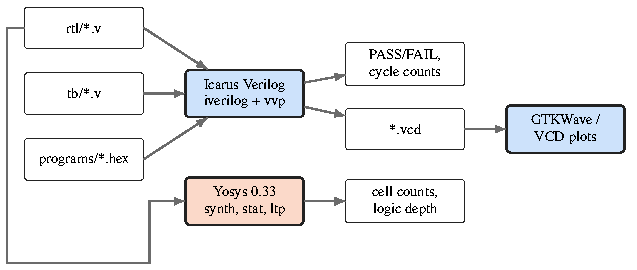
\includegraphics[width=\columnwidth]{toolchain.pdf}
\caption{Tool flow: Icarus Verilog for simulation, VCD/GTKWave for waveforms, Yosys for generic synthesis.}
\label{fig:toolchain}
\end{figure}

\begin{figure}[!t]
\centering
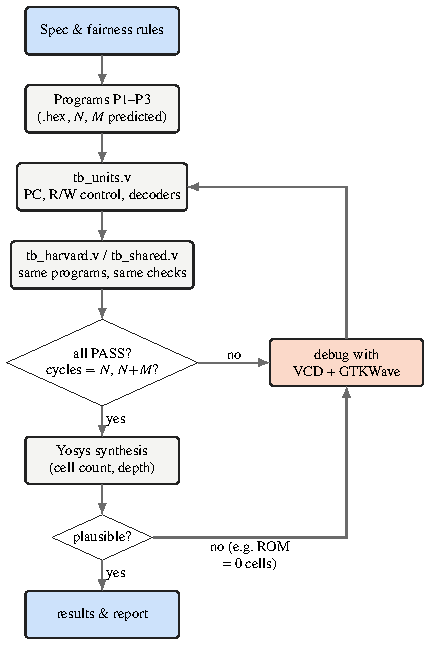
\includegraphics[width=0.6\columnwidth]{verif_flow.pdf}
\caption{Verification flow. Synthesis output is itself checked for plausibility, which is how the bug in Section~\ref{sec:mismatch} was found.}
\label{fig:verif}
\end{figure}

\begin{figure*}[!t]
\centering
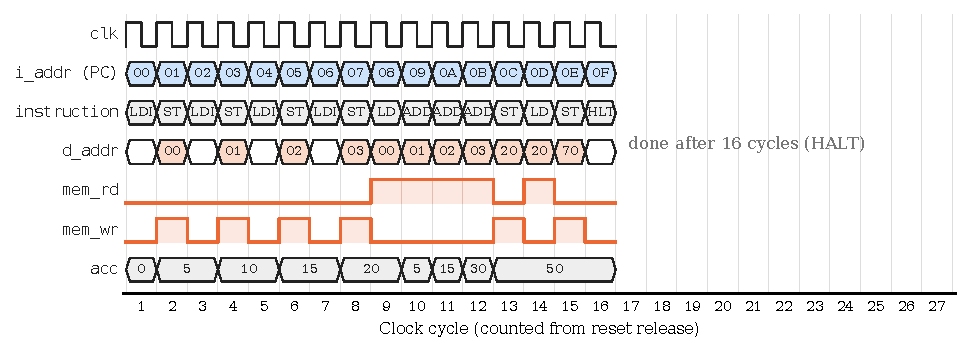
\includegraphics[width=\textwidth]{wave_harvard.pdf}\\[-1mm]
{\footnotesize (a) Harvard, 16 cycles: \sig{i\_addr} advances every cycle while \sig{mem\_rd}/\sig{mem\_wr} are active in the \emph{same} cycles.}\\[2mm]
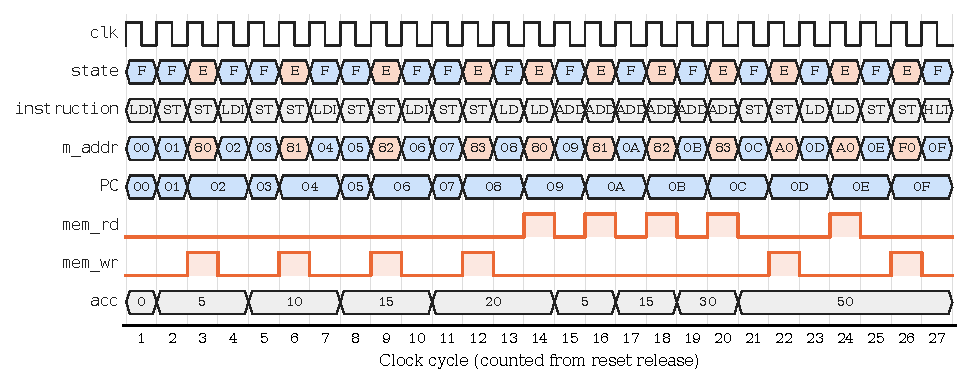
\includegraphics[width=\textwidth]{wave_shared.pdf}\\[-1mm]
{\footnotesize (b) Shared, 27 cycles: each LOAD/STORE/ADD takes a FETCH cycle (F, \sig{m\_addr}~=~PC) and an EXEC cycle (E, \sig{m\_addr}~=~\texttt{0x80}+offset); LDI and HALT finish in FETCH.}
\caption{Simulated waveforms for program P2 (array sum), plotted from the VCD files at the same cycle width.}
\label{fig:waveh}
\end{figure*}

% ------------------------------------------------------------------
\section{Results}\label{sec:results}

\subsection{Functional correctness}
Both designs produce identical final state on all three programs: P1 copies \{11,\,22,\,33,\,44\} and outputs 44; P2 computes $5{+}10{+}15{+}20=50$, stores it, reads it back and outputs 50; P3 outputs 3, and its write to unmapped offset \texttt{0x90} is blocked in both designs. In the shared design this also protects program word \texttt{0x10}.

\subsection{Cycle counts and speed-up}
Table~\ref{tab:cycles} and Fig.~\ref{fig:cycles} give the measured counts. Every count equals the prediction of~\eqref{eq:model} exactly. Fig.~\ref{fig:speedup} places the three measured speed-ups on the line $S=1+f$. For comparison it also shows the flat $2\times$ that a baseline charging EXEC on every instruction would report regardless of the program. Fig.~\ref{fig:occ} shows cycle by cycle, for P2, where the 11 extra cycles come from: the Harvard data bus is busy in 11 of 16 cycles, and in the shared design each of those 11 data accesses needs a cycle of its own on the single port.

\begin{table}[!t]
\caption{Measured cycle counts (Icarus Verilog)}
\label{tab:cycles}
\centering
\begin{tabular}{@{}lcccccc@{}}
\toprule
Program & $N$ & $M$ & $f$ & $T_H$ & $T_S$ & $S$ \\
\midrule
P1 block copy     & 18 & 13 & 0.72 & 18 & 31 & 1.72 \\
P2 array sum      & 16 & 11 & 0.69 & 16 & 27 & 1.69 \\
P3 compute-heavy  & 16 &  4 & 0.25 & 16 & 20 & 1.25 \\
\bottomrule
\end{tabular}
\end{table}

\begin{figure}[!t]
\centering
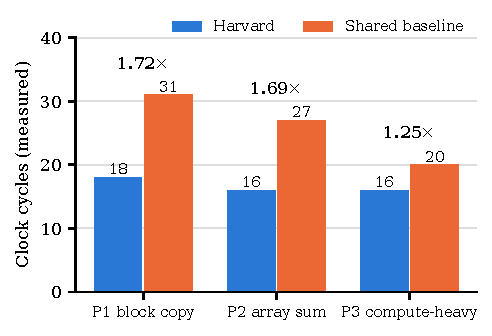
\includegraphics[width=\columnwidth]{cycles.pdf}
\caption{Measured clock cycles per program, with speed-up $T_S/T_H$.}
\label{fig:cycles}
\end{figure}

\begin{figure}[!t]
\centering
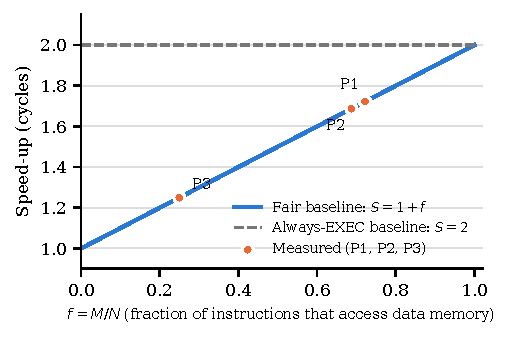
\includegraphics[width=\columnwidth]{speedup.pdf}
\caption{Speed-up versus the fraction of data-memory instructions $f$. Measured points lie exactly on the fair-baseline model $S=1+f$.}
\label{fig:speedup}
\end{figure}

\begin{figure*}[!t]
\centering
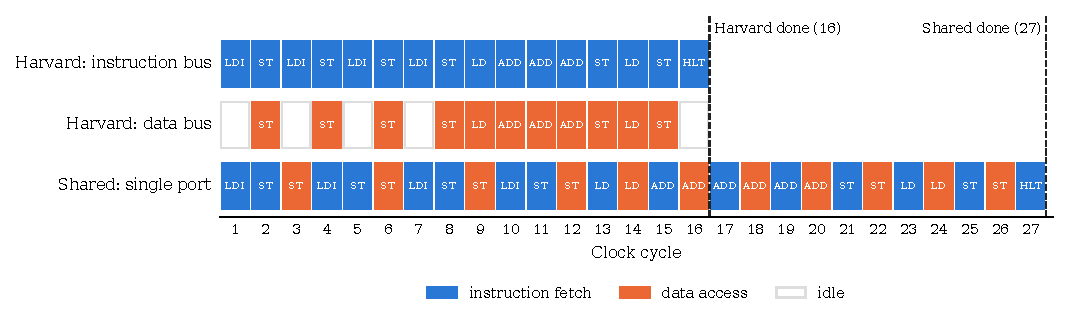
\includegraphics[width=0.95\textwidth]{bus_occupancy.pdf}
\caption{Bus occupancy per cycle for P2, derived from the simulation VCD. The Harvard instruction and data buses work in parallel. On the shared port, fetches (blue) and data accesses (orange) are serialized.}
\label{fig:occ}
\end{figure*}

\subsection{Generic synthesis}
Table~\ref{tab:synth} summarizes Yosys~0.33 generic synthesis (\texttt{synth}, program P2). Both designs are dominated by a $256\times32$ storage array of 8\,192 enable flip-flops plus its read multiplexer (16\,912 cells). Outside that array the logic is small and similar (Fig.~\ref{fig:synth}). Two details are informative. The Harvard ROM costs only 39 cells, because its contents are constant and are folded into logic. The shared design has 86 rather than 73 other flip-flops: its 32-bit IR keeps only the 12 bits it uses (opcode and address), because LDI completes in FETCH and the immediate field is never read from IR, so Yosys removes the other 20 bits.

\begin{table}[!t]
\caption{Generic synthesis results (Yosys 0.33, program P2)}
\label{tab:synth}
\centering
\begin{tabular}{@{}lrr@{}}
\toprule
 & Harvard & Shared \\
\midrule
Total cells                      & 17\,481 & 17\,471 \\
\quad memory array (DFFE)        & 8\,192  & 8\,192 \\
\quad memory read/write logic    & 8\,720  & 8\,720 \\
\quad instruction ROM            & 39      & --- \\
\quad controller                 & 384     & 368 \\
\quad decoder                    & 15      & 16 \\
\quad PC, OUT, R/W ctrl, glue    & 131     & 175 \\
Other flip-flops (SDFFE)         & 73      & 86 \\
Longest path (gate levels)       & 33      & 31 \\
Maximum frequency                & \multicolumn{2}{c}{not measured (Phase II)} \\
\bottomrule
\end{tabular}
\end{table}

\begin{figure}[!t]
\centering
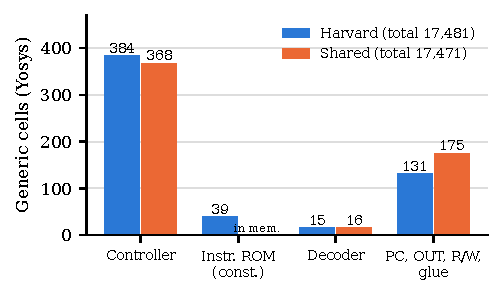
\includegraphics[width=\columnwidth]{synth_logic.pdf}
\caption{Cells outside the shared $256\times32$ storage array. In the shared design the program lives in the RAM, so it has no separate ROM.}
\label{fig:synth}
\end{figure}

\subsection{Critical path}\label{sec:cp}
We measured the longest combinational path with Yosys (\texttt{flatten; ltp -noff}, one unit per cell). Fig.~\ref{fig:cp} shows the result. The Harvard path runs PC $\rightarrow$ ROM read $\rightarrow$ RAM read $\rightarrow$ 32-bit add $\rightarrow$ ACC: 33 levels, because \emph{two} memory reads are chained in one cycle. The shared path starts at IR, so only \emph{one} memory read is on it: 31 levels. This matches the textbook trade-off~\cite{patterson,harris}. The single-cycle Harvard design saves cycles but pays with a longer cycle. With these unit-delay figures, the Harvard design would still win in execution time whenever $1+f > 33/31 \approx 1.06$, that is, for $f > 0.06$. Unit-delay depth is not real timing, however, so this is an indication only (Section~\ref{sec:discussion}).

\begin{figure}[!t]
\centering
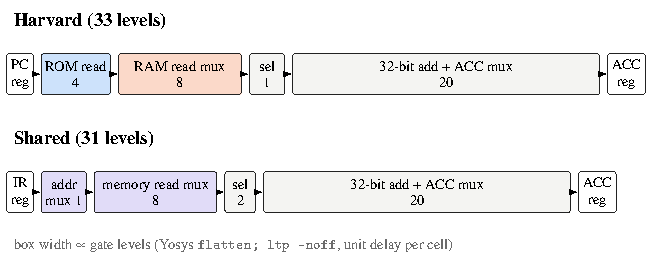
\includegraphics[width=\columnwidth]{critical_path.pdf}
\caption{Longest register-to-register paths reported by Yosys. Harvard chains an instruction read and a data read; shared has a single memory read per cycle.}
\label{fig:cp}
\end{figure}

\subsection{A simulation/synthesis mismatch}\label{sec:mismatch}
An early version filled the ROM with HALT words in a \texttt{for} loop before calling \sig{\$readmemh}. Icarus executes these in source order, so simulation was correct. Yosys, however, applied the file contents first and the loop afterwards. The synthesized ROM held only HALT words and was optimized to zero cells. The plausibility check in Fig.~\ref{fig:verif} caught this, and the loop was removed. This is a concrete instance of the mismatch class described in~\cite{mills}, and it is why we check every synthesis number for plausibility before reporting it.

% ------------------------------------------------------------------
\section{Discussion and Limitations}\label{sec:discussion}
\textbf{Simultaneous access opportunities.} The brief asks us to analyse when separate paths help. Our answer is quantitative. A separate data path saves exactly one cycle for every instruction that accesses data memory, and nothing for any other instruction. The benefit therefore scales with $f$. Memory-heavy kernels such as copies and reductions gain about $1.7\times$, while compute-heavy code gains much less.

\textbf{Speed-up is in cycles, not time.} We have not run place-and-route, so we report no maximum frequency. The 33 vs.\ 31 gate-level depth suggests that the Harvard cycle is slightly longer, and the true ratio depends on memory and adder delays on a real device.

\textbf{Area similarity is largely a sizing choice.} Both designs instantiate one $256\times32$ array. Harvard gives all of it to data, of which only 112 words are addressable, and puts the program in a constant ROM. Shared splits the array into 128 program words and 112 data words. With different sizes, or with a writable instruction memory, the area comparison would change. The near-equal totals should not be read as ``Harvard costs nothing extra.''

\textbf{Combinational-read memories.} The single-cycle Harvard design depends on memories that return data in the same cycle. FPGA block RAM reads synchronously~\cite{ug473}, so our memories synthesize to flip-flops. This is acceptable at $256\times32$ but does not scale.

\textbf{Neither design is pipelined.} The shared design's extra cycle comes from a resource conflict on one memory port. We do not call it a structural \emph{hazard}, because that term describes overlapping instructions in a pipeline, and our designs do not overlap instructions.

\textbf{Scope of evidence.} We used three hand-written programs, single-cycle memory latency, no caches, and no shared lower-level memory. The results support the cycle model above and nothing broader.

% ------------------------------------------------------------------
\section{Individual Contributions}\label{sec:contrib}
Work was divided into five packages, and each package was committed to the repository under its owner's name. All members reviewed the integrated design and the comparison rules.

\begin{table}[h]
\caption{Work packages and owners}
\label{tab:contrib}
\centering
\small
\begin{tabular}{@{}p{1.85cm}p{5.85cm}@{}}
\toprule
Member & Contribution \\
\midrule
Aabir Sarkar & WP1 Memories: \sig{instr\_rom}, \sig{data\_ram}, \sig{out\_reg}, \sig{shared\_mem}; test programs P1--P3; the \sig{\$readmemh} ROM fix. \\
Kush Puri & WP2 Control glue: \sig{pc}, \sig{rw\_control}, \sig{harvard\_decoder}, \sig{shared\_decoder}; unit testbench \sig{tb\_units}. \\
Kavya Katal & WP3 Harvard core and integration: \sig{harvard\_ctrl}, \sig{harvard\_top}, Harvard block diagram; repository, README, module documentation and report integration. \\
Kushagra Maheshwari & WP4 Shared baseline: \sig{shared\_ctrl} FETCH/EXEC FSM, \sig{shared\_top}, shared block diagram, fair-baseline cycle rule. \\
Aadit Vachher & WP5 Verification and results: \sig{tb\_harvard}, \sig{tb\_shared}, \sig{run\_all.sh}, Yosys scripts, results analysis. \\
\bottomrule
\end{tabular}
\end{table}

% ------------------------------------------------------------------
\section{Conclusion and Future Work}
We implemented a Harvard-style memory organization and a fair shared-memory baseline in modular, synthesizable Verilog. The two designs differ only in memory organization, and both were verified with 71 directed checks. Cycle counts follow $T_H=N$ and $T_S=N+M$ exactly, giving speed-ups of $1.25\times$ to $1.72\times$ that grow with the fraction of instructions that access data. The cost is a slightly deeper single-cycle path, because an instruction read and a data read are chained. Generic synthesis area is similar for the chosen memory sizes.

Phase~II will turn the cycle result into a time result and widen the evidence: (i)~synchronous-read memories that map to block RAM, used in both designs; (ii)~place-and-route on a chosen FPGA (e.g.\ iCE40 with \texttt{nextpnr}) to measure $f_\text{max}$ and real resource use; (iii)~a program sweep across $f\in[0,1]$, including larger generated kernels; (iv)~multi-cycle memory latency, where separate paths should matter more; (v)~the optional shared lower-level memory behind split instruction/data memories, a modified-Harvard organization; and (vi)~a dual-ported shared memory as a third baseline, to separate the effect of port count from that of separate storage.

% ------------------------------------------------------------------
\begin{thebibliography}{99}
\bibitem{vonneumann} J.~von Neumann, ``First draft of a report on the EDVAC,'' Moore School of Electrical Engineering, Univ. of Pennsylvania, 1945; reprinted in \emph{IEEE Ann. Hist. Comput.}, vol.~15, no.~4, pp.~27--75, 1993.
\bibitem{backus} J.~Backus, ``Can programming be liberated from the von Neumann style? A functional style and its algebra of programs,'' \emph{Commun. ACM}, vol.~21, no.~8, pp.~613--641, Aug. 1978.
\bibitem{aiken} H.~H.~Aiken and G.~M.~Hopper, ``The automatic sequence controlled calculator,'' \emph{Electrical Engineering}, vol.~65, pp.~384--391, 449--454, 522--528, 1946.
\bibitem{eyre} J.~Eyre and J.~Bier, ``The evolution of DSP processors,'' \emph{IEEE Signal Process. Mag.}, vol.~17, no.~2, pp.~43--51, Mar. 2000.
\bibitem{hennessy} J.~L.~Hennessy and D.~A.~Patterson, \emph{Computer Architecture: A Quantitative Approach}, 6th~ed. Cambridge, MA, USA: Morgan Kaufmann, 2017.
\bibitem{smith} A.~J.~Smith, ``Cache memories,'' \emph{ACM Comput. Surv.}, vol.~14, no.~3, pp.~473--530, Sep. 1982.
\bibitem{patterson} D.~A.~Patterson and J.~L.~Hennessy, \emph{Computer Organization and Design: The Hardware/Software Interface}, 5th~ed. Waltham, MA, USA: Morgan Kaufmann, 2014.
\bibitem{harris} D.~M.~Harris and S.~L.~Harris, \emph{Digital Design and Computer Architecture}, 2nd~ed. Waltham, MA, USA: Morgan Kaufmann, 2012.
\bibitem{wulf} W.~A.~Wulf and S.~A.~McKee, ``Hitting the memory wall: Implications of the obvious,'' \emph{ACM SIGARCH Comput. Archit. News}, vol.~23, no.~1, pp.~20--24, Mar. 1995.
\bibitem{amdahl} G.~M.~Amdahl, ``Validity of the single processor approach to achieving large scale computing capabilities,'' in \emph{Proc. AFIPS Spring Joint Comput. Conf.}, 1967, pp.~483--485.
\bibitem{ieee1364} \emph{IEEE Standard for Verilog Hardware Description Language}, IEEE Std 1364-2005, 2006.
\bibitem{palnitkar} S.~Palnitkar, \emph{Verilog HDL: A Guide to Digital Design and Synthesis}, 2nd~ed. Upper Saddle River, NJ, USA: Prentice Hall, 2003.
\bibitem{mills} D.~Mills and C.~E.~Cummings, ``RTL coding styles that yield simulation and synthesis mismatches,'' in \emph{Proc. SNUG}, San Jose, CA, USA, 1999.
\bibitem{ug473} Xilinx, \emph{7 Series FPGAs Memory Resources User Guide}, UG473.
\bibitem{icarus} S.~Williams, ``Icarus Verilog.'' [Online]. Available: \url{https://steveicarus.github.io/iverilog/}
\bibitem{gtkwave} T.~Bybell, ``GTKWave.'' [Online]. Available: \url{https://gtkwave.sourceforge.net/}
\bibitem{yosys} C.~Wolf, ``Yosys Open SYnthesis Suite.'' [Online]. Available: \url{https://yosyshq.net/yosys/}
\end{thebibliography}

\end{document}
